\section{Experiments}

This section details the experimental methodology employed to evaluate the effectiveness of PhyPrompt on physics-driven video generation tasks. Our assessment focuses on three primary aspects: (1) the physical plausibility and semantic fidelity of the generated videos, (2) the transferability of the learned PhyPrompt rewriter across diverse text-to-video (T2V) generators, and (3) ablation studies investigating the contributions of key components within our proposed approach.
\\
\textbf{Text-to-Video Generators.}
PhyPrompt's performance is evaluated using several state-of-the-art T2V diffusion models, with parameter counts ranging from 860 million to 5 billion:

\begin{itemize}
\item \textbf{Lavie}~\cite{wang2023lavie}: An 860M-parameter model that utilizes cascaded latent diffusion, trained on the Vimeo25M dataset. It is capable of generating videos up to 8 seconds in length at a 1280×720 pixel resolution.
\item \textbf{VideoCrafter2}~\cite{chen2024videocrafter2}: This 1.2B-parameter model employs a diffusion-based architecture. It was trained using a combination of low-quality videos and high-quality images to improve motion consistency and visual fidelity, producing videos up to 8 seconds in duration at a 512×512 resolution.
\item \textbf{CogVideoX-2B}~\cite{yang2024cogvideox}: A 2B-parameter model featuring a 3D variational autoencoder and an expert transformer with adaptive LayerNorm. It generates videos up to 6 seconds long at a 720×480 resolution.
\item \textbf{CogVideoX-5B}~\cite{yang2024cogvideox}: This 5B-parameter model shares the architecture of CogVideoX-2B but benefits from larger-scale training data. It produces videos up to 6 seconds in length at a 720×480 resolution.
\end{itemize}
To ensure consistent evaluation across all models, generated videos were standardized to a duration of 6 seconds, a frame rate of 4 FPS, and a resolution of 720×480 pixels. Detailed configurations of the T2V generation setup are provided in supplementary material.
\\
\textbf{Prompt Enhancer.}
PhyPrompt variants are obtained by fine‑tuning Qwen2.5‑Instruct checkpoints with 1.5B, 3B, and 7B parameters.
For comparison we include four automatic prompt‑refinement baselines: Promptist~\cite{hao2023promptist}, PhyT2V~\cite{xue2024phyt2v}, GPT‑4o~\cite{achiam2023gpt-4o}, and DeepSeek‑V3~\cite{liu2024deepseek-v3}.
\\
\textbf{Dataset.}
Our approach is evaluated on the VideoPhy2 benchmark~\cite{bansal2025videophy2}. This benchmark comprises a diverse collection of prompts specifically designed to assess physical commonsense in video generation, encompassing scenarios related to gravity, collisions, fluid dynamics, and other fundamental physical phenomena.
\\
\textbf{Evaluation Metrics.}
Consistent with~\cite{bansal2025videophy2}, generated videos are assessed based on two criteria: semantic adherence (SA) and physical commonsense (PC). Each criterion is evaluated on a 5-point Likert scale, ranging from Very Unlikely (1) to Very Likely (5). We random sample 500 prompts from the test set and report the percentage of generated videos satisfying the following conditions:
\begin{itemize}
\item \textbf{Semantic Adherence (SA $\geq$ 4)}: The percentage of videos that accurately depict the intended content described in the prompt.
\item \textbf{Physical Commonsense (PC $\geq$ 4)}: The percentage of videos that realistically adhere to fundamental physical principles.
\item \textbf{Joint Performance (SA $\geq$  4 and PC $\geq$  4)}: The percentage of videos that concurrently achieve high scores (i.e., $\geq$ 4) in both semantic adherence and physical realism.
\end{itemize}

\subsection{Quality Assessment of Generated Videos}
\label{sec:quality}
We measure how well each prompt-rewriting strategy improves \textbf{semantic adherence (SA)} and \textbf{physical commonsense (PC)} when paired with \textbf{CogVideoX-2B}\cite{yang2024cogvideox}.
Table\ref{tab:quality} reports results on 500 prompts from the \textsc{VideoPhy2} benchmark~\cite{bansal2025videophy2}.

\begin{table*}
\centering
\caption{\textbf{VideoPhy2 quality results with CogVideoX-2B.}
For each prompt-rewriting strategy we report the percentage of videos scoring $\ge\!4$ for semantic adherence (SA) and physical commonsense (PC), their joint percentage (SA \& PC), and the average SA/PC scores (Avg SA, Avg PC).}
\vspace{0.1in}
\label{tab:quality}
\setlength{\tabcolsep}{3mm}{
\renewcommand\arraystretch{0.9}
\resizebox{\linewidth}{!}{
\begin{tabular}{lccccc}
\toprule
\textbf{Enhanced Model} &
\textbf{SA (\%)} $\uparrow$ &
\textbf{PC (\%)} $\uparrow$ &
\textbf{SA \& PC (\%)} $\uparrow$ &
\textbf{Avg SA} $\uparrow$ &
\textbf{Avg PC} $\uparrow$ \\
\midrule
N/A (Original Prompt)           & 43.4 & 55.8 & 32.2 & 3.842 & 4.410 \\
Promptist~\cite{hao2023promptist}     & 41.2 & 58.2 & 30.2 & 3.782 & 4.452 \\
PhyT2V~\cite{xue2024phyt2v}     & 45.0 & 62.0 & 36.2 & 3.854 & 4.522 \\
\midrule
Qwen2.5-1.5B              & 37.6 & 64.0 & 31.8 & 3.616 & 4.562 \\
PhyPrompt-1.5B            & 42.8 & 65.4 & 37.4 & 3.800 & 4.580 \\
\addlinespace[4pt]
Qwen2.5-3B                & 40.0 & 64.2 & 32.0 & 3.754 & 4.582 \\
PhyPrompt-3B              & 46.4 & 64.8 & 39.6 & 3.868 & 4.556 \\
\addlinespace[4pt]
Qwen2.5-7B                & 44.8 & 64.6 & 34.2 & 3.848 & 4.586 \\
PhyPrompt-7B              & 47.8 & \textbf{66.8} & \textbf{40.8} & 3.878 & \textbf{4.590} \\
\midrule
GPT-4o                    & 47.0 & 60.0 & 37.0 & 3.932 & 4.488 \\
DeepSeek-V3               & \textbf{48.4} & 64.6 & 38.6 & \textbf{3.968} & 4.564 \\
\bottomrule
\end{tabular}%
}}
\end{table*}

\noindent \textbf{Effectiveness of PhyPrompt.}
Promptist~\cite{hao2023promptist} raises PC from 55.8\% to 58.2\% but drops SA from 43.4\% to 41.2\%, causing its joint score to fall from 32.2\% to 30.2\%, confirming that a generic text-to-image adapter does not reliably balance semantics and physics in the video domain. PhyT2V~\cite{xue2024phyt2v} achieves 45.0\% SA and 62.0\% PC (36.2\% joint), demonstrating the value of iterative LLM feedback, but requires multiple prompting rounds and complex step-back mechanisms. In contrast, all three PhyPrompt checkpoints outperform both the original prompts and existing baselines on every metric. The 7B model delivers the largest gains with SA 47.8\%, PC 66.8\%, and a joint success rate of 40.8\%, representing an absolute improvement of +8.6\% over the baseline and +10.6\% over Promptist. Notably, even the 1.5B variant achieves a 37.4\% joint score, surpassing Promptist by +7.2\% while using only 1/10 the parameters of GPT-4o. The consistent improvements across all model sizes validate the effectiveness of our two-stage training approach combining physics-focused SFT with dynamic reward-based RL.

\noindent\textbf{Advantages over general-purpose large language models.}
PhyPrompt demonstrates that domain-specialized training outperforms raw parameter scaling for physics-aware video generation. Compared to GPT-4o~\cite{achiam2023gpt-4o}, PhyPrompt-7B achieves nearly identical SA (47.8\% vs 47.0\%) while delivering substantially higher PC (66.8\% vs 60.0\%) and joint performance (40.8\% vs 37.0\%). This +6.8\% PC advantage stems from three factors: (i) end-to-end RL optimization on video quality metrics rather than text likelihood~\cite{ouyang2022training}, (ii) physics-focused CoT pretraining that encodes domain-specific reasoning~\cite{wei2022chain}, and (iii) dynamic reward curricula that balance dual objectives~\cite{bengio2009curriculum}. DeepSeek-V3~\cite{liu2024deepseek-v3}, despite 100× more parameters (671B), trails PhyPrompt-7B in PC (64.6\% vs 66.8\%) and joint performance (38.6\% vs 40.8\%), confirming that general-purpose pretraining does not substitute for task-specific feedback~\cite{hoffmann2022training}. PhyPrompt-3B matches GPT-4o using less than 1\% of its parameters, exemplifying recent findings that specialized smaller models can surpass general larger ones on focused tasks~\cite{muennighoff2023scaling}. Overall, our results align with emerging evidence that domain-targeted training with direct task feedback provides a more parameter-efficient path than scaling alone~\cite{kaplan2020scaling,wei2022emergent}.


\subsection{Zero-Shot Transfer Across Generators}
\label{sec:transfer}
\begin{figure*}[t]
    \centering
   \resizebox{1.0\textwidth}{!}{%
    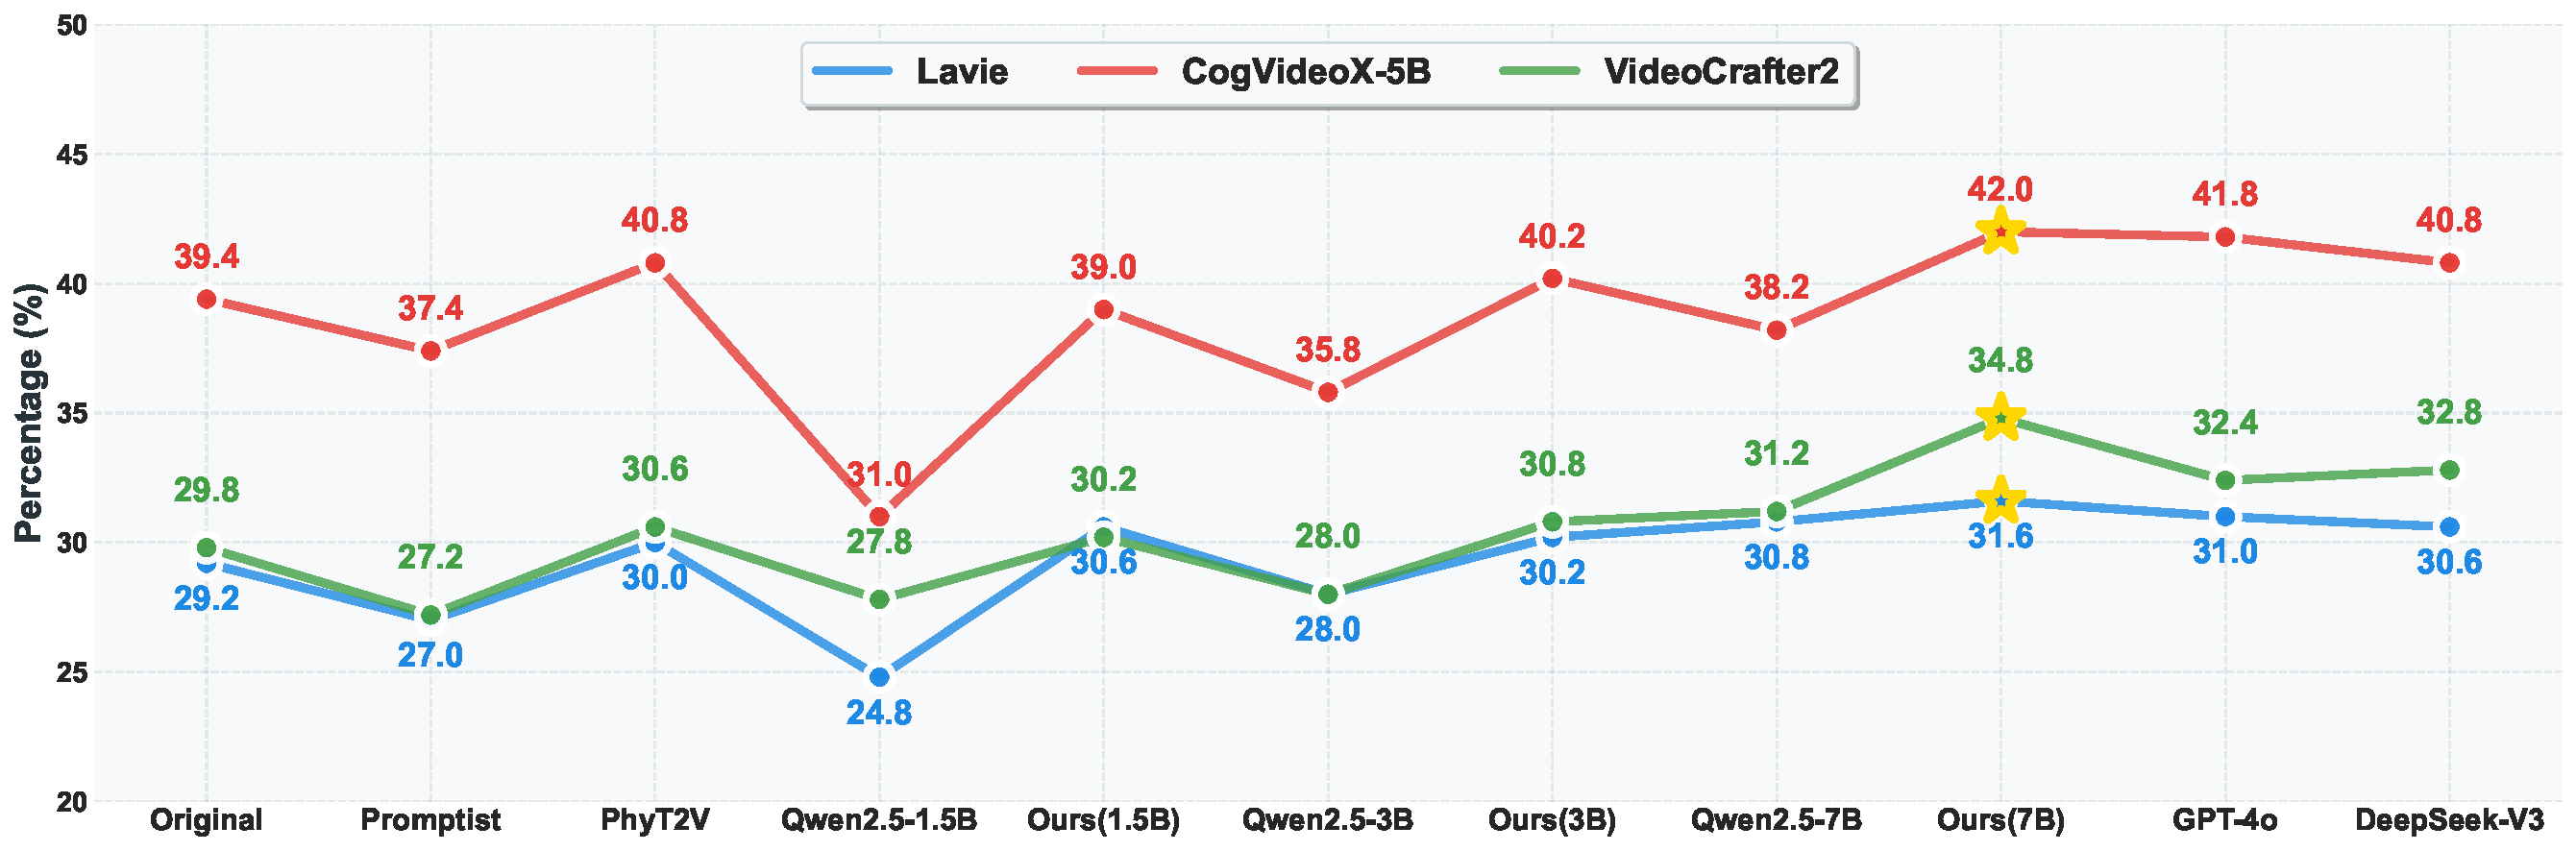
\includegraphics{figures/all_results_combined.pdf}
    }
    \vspace{-0.15in}
    \caption{\textbf{Cross-Generator Transfer of PhyPrompt.} Performance comparison across different prompt enhancement methods on three text-to-video generation models (Lavie, CogVideoX-5B, and VideoCrafter2) measured by joint Physical Commonsense and Semantic Adherence (PC \& SA) metrics. Our method consistently outperforms baseline approaches (Original, Promptist, PhyT2V) and similarly-sized Qwen2.5 models across all three video generation backbends. The highest performance (42.0\%) is achieved by our 7B model on CogVideoX-5B. Gold stars indicate the best-performing method for each generator.}
    \label{fig:transfer}
    \vspace{-0.2in}
\end{figure*}

\begin{figure}[!htbp]
  \centering
    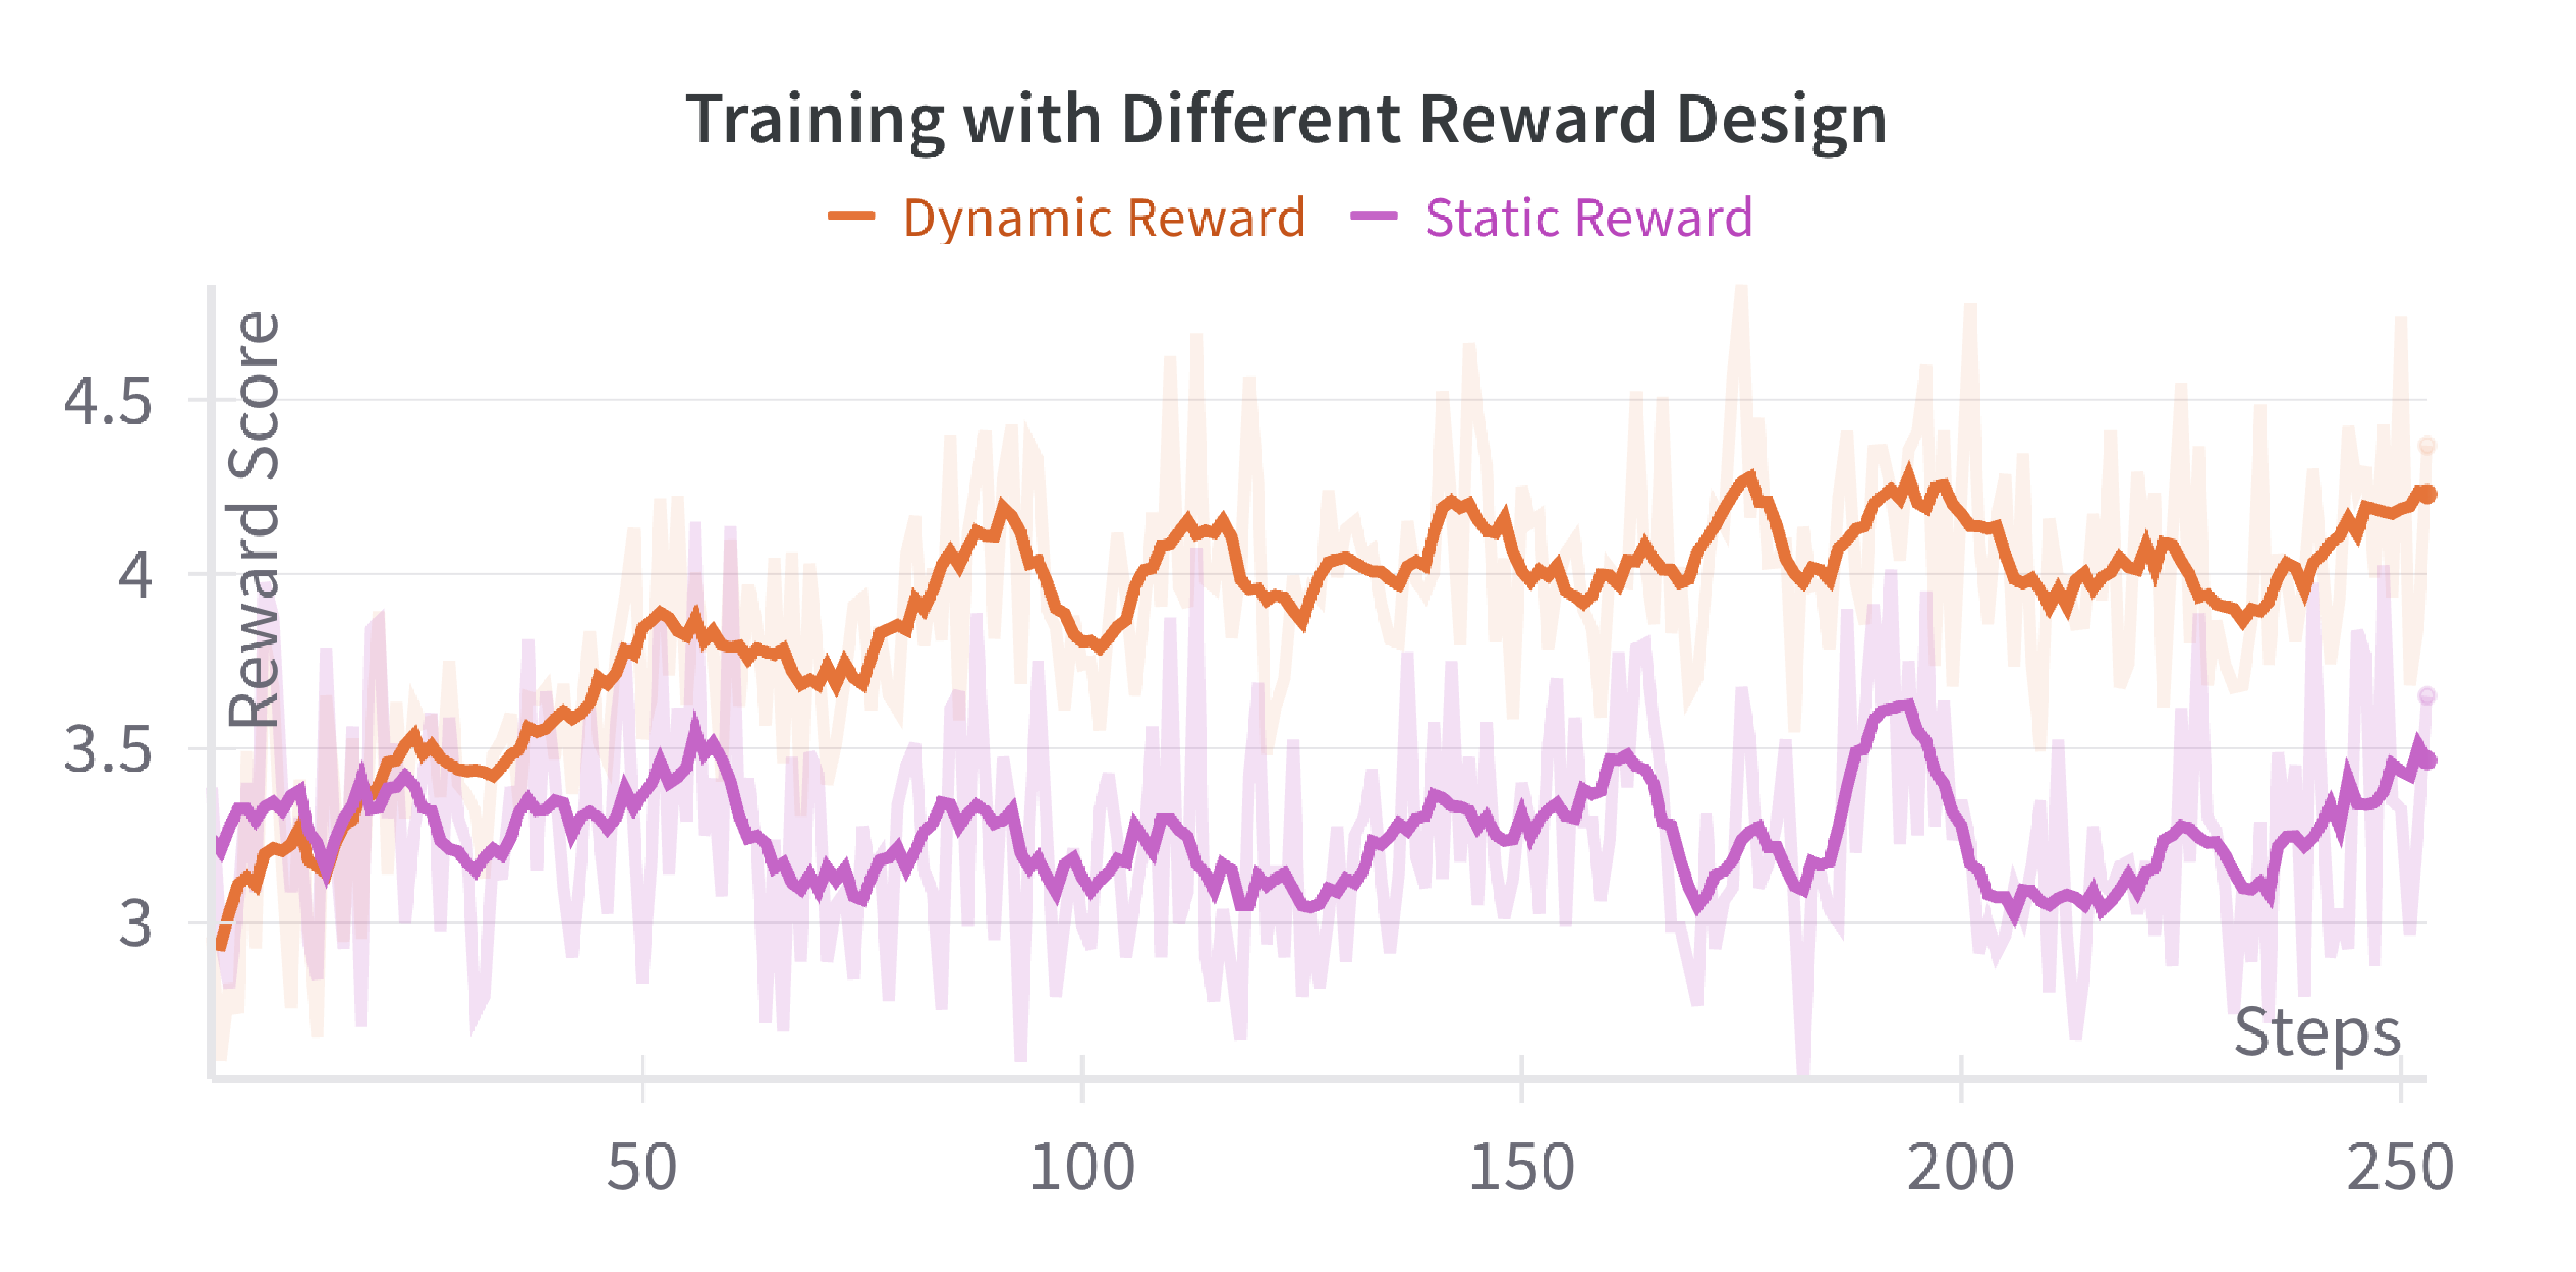
\includegraphics[width=1.0\linewidth]{figures/reward.pdf}
    \captionof{figure}{Training reward curves under the dynamic (orange) and static (purple) reward formulations. Each line is smoothed with a 10-step moving average; lightly shaded traces show the unsmoothed per-episode rewards. The dynamic curriculum converges more rapidly and plateaus higher (4.2) than the static baseline (3.5), indicating more effective optimization.}
    \label{fig:reward_curve}
  \vspace{-1em}
\end{figure}

To verify PhyPrompt's generator-agnostic transfer, we evaluate PhyPrompt-7B (trained solely on CogVideoX-2B) on three architecturally diverse diffusion models: Lavie (860M), VideoCrafter2 (1.2B), and CogVideoX-5B (5B). We generate 500 videos per method for each generator and report joint SA\&PC scores in~\cref{fig:transfer}. Full results appear in the supplement.

\noindent\textbf{Joint-metric improvement.} Original prompts achieve baseline joint scores of 29.2\% (Lavie), 29.8\% (VideoCrafter2), and 39.4\% (CogVideoX-5B). Promptist degrades performance to 27.0\%, 27.2\%, and 37.4\%, respectively. PhyPrompt substantially surpasses baselines on every generator: Lavie reaches 31.6\% (+8.2\% over original), VideoCrafter2 achieves 34.8\% (+16.8\% over original), and CogVideoX-5B attains 42.0\% (+6.6\% over original). Smaller PhyPrompt variants (1.5B and 3B) exhibit the same improvement pattern, with the 3B model achieving 30.2\%, 30.8\%, and 40.2\% respectively, confirming that our training approach scales effectively across model sizes.

\noindent\textbf{Comparison with other rewriters.} PhyT2V shows improvements over Promptist but underperforms PhyPrompt across all generators, achieving 30.0\%, 30.6\%, and 40.8\% on Lavie, VideoCrafter2, and CogVideoX-5B respectively. GPT-4o, DeepSeek-V3, and size-matched Qwen baselines similarly trail PhyPrompt on the joint metric. On VideoCrafter2, the best alternative (DeepSeek-V3, 32.8\%) remains 2.0\% below PhyPrompt-7B; similar margins hold on Lavie and CogVideoX-5B.

\noindent\textbf{Zero-shot transfer.} All PhyPrompt variants are fine-tuned solely on CogVideoX-2B outputs yet yield substantial gains on Lavie and VideoCrafter2 without any back-end adjustment. This confirms genuine zero-shot transfer where physics-aware rewrites capture model-agnostic physical priors rather than exploiting generator-specific biases. Related work in parameter-efficient prompt tuning for language models has similarly demonstrated cross-model generalization~\cite{lester2021power,li2021prefix}, and RL-based prompt adapters have been shown to transfer across modalities~\cite{hao2023promptist}. By disentangling physical constraints from any particular diffusion architecture, PhyPrompt removes the need for per-generator fine-tuning, cutting computational overhead and enabling rapid deployment across diverse T2V pipelines.



\subsection{Ablation Study}
To disentangle the sources of PhyPrompt’s gains, we conduct two complementary ablations.
First, we examine how the choice of reward schedule during GRPO fine‑tuning shapes performance.
Second, we test the necessity of the two‑stage pipeline (SFT and RL).
Results show that both the curriculum reward and the two‑stage procedure contribute sizable, complementary improvements.

\subsubsection{Reward Design}
\label{sec:reward_design}

\begin{figure*}[!htbp]
  \centering
  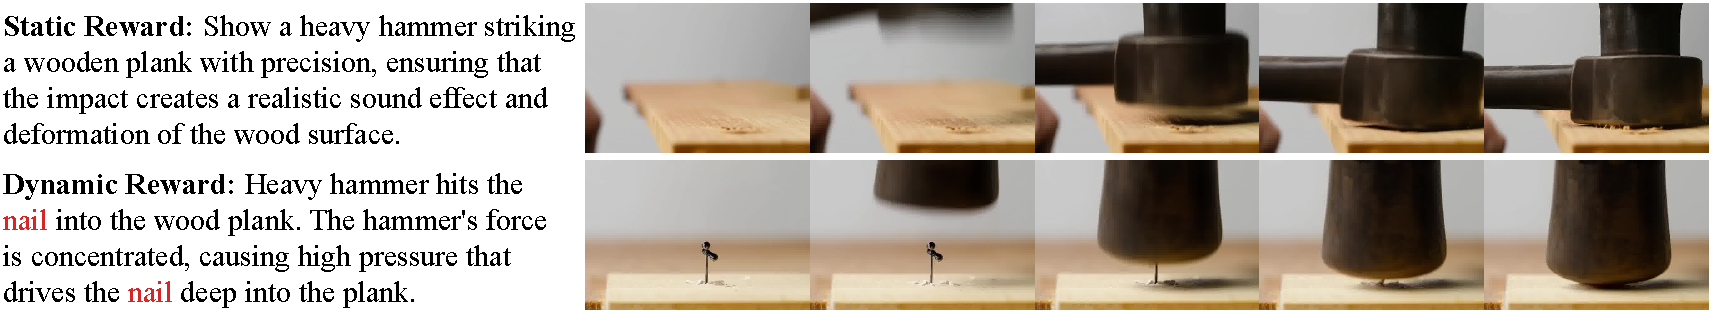
\includegraphics[width=\textwidth]{figures/reward_demo.pdf}
   \caption{\textbf{Frame‐by‐frame comparison of CogVideoX-2B outputs for the “hammer and nail” scenario.}
Top row shows results using the static‐reward prompt
“\textit{Show a heavy hammer striking a wooden plank with precision, ensuring that the impact creates a realistic sound effect and deformation of the wood surface.}”
The hammer impacts the plank but no nail is visible or driven.
Bottom row shows results using the dynamic‐reward prompt
“\textit{Heavy hammer hits the nail into the wood plank. The hammer’s force is concentrated, causing high pressure that drives the nail deep into the plank.}”
Here the nail appears in frame 1, is pressed gradually into the wood across frames 2–3, and achieves full penetration by frame 4, with realistic wood deformation and depth of entry.}
\vspace{-1em}
  \label{fig:hammer_frames}
\end{figure*}

To demonstrate that semantic adherence (SA) and physical commonsense (PC) are inherently conflicting objectives, we conduct a systematic ablation comparing four reward strategies: (i)~SA-only optimization ($w_{\text{sa}} = 1.0, w_{\text{pc}} = 0.0$), (ii)~PC-only optimization ($w_{\text{sa}} = 0.0, w_{\text{pc}} = 1.0$), (iii)~static balanced weighting ($w_{\text{sa}} = w_{\text{pc}} = 0.5$), and (iv)~our dynamic curriculum (Eq.~\ref{eq:total_reward}). We use Qwen2.5-7B-Instruct as the base model and CogVideoX-2B as the video generator. Results are shown in \cref{fig:reward_curve} and~\cref{tab:reward_ablation}.

\noindent\textbf{Negative Transfer Between Objectives.}
\cref{tab:reward_ablation} reveals severe negative transfer. SA-only training improves semantic adherence to 45.6\% (+2.2\% over baseline) but degrades physical commonsense to 52.8\% ($-3.0\%$), yielding worse joint performance (31.6\% vs. 32.2\% baseline). Conversely, PC-only training achieves 65.2\% physics score (+9.4\%) but drops semantic adherence to 39.4\% ($-4.0\%$), with only marginal joint improvement (33.4\%). This antagonistic relationship demonstrates that SA and PC cannot be jointly maximized through naive single-objective optimization. Static balanced weighting achieves 35.4\% joint success, superior to either extreme but still 5.4\% below our dynamic curriculum.

\noindent\textbf{Dynamic Curriculum Exceeds Single-Objective Upper Bounds.}
Our dynamic curriculum achieves SA = 47.8\% and PC = 66.8\%. Remarkably, this outperforms SA-only training on semantic adherence (47.8\% vs. 45.6\%) and simultaneously outperforms PC-only training on physical commonsense (66.8\% vs. 65.2\%). In other words, our method beats each specialist on its own objective. This indicates that optimizing both objectives together with a curriculum yields better results than optimizing either objective alone~\cite{caruana1997multitask,yu2020gradient,standley2020tasks}.


We hypothesize that semantic descriptions establish object identities and relationships (e.g., "a ball" and "an incline"), while physical constraints refine these with dynamics (e.g., "accelerates" and "under gravity"). High-quality physical descriptions require precise semantic grounding~\cite{scholkopf2021toward}: one cannot specify realistic forces without first establishing what objects exist. SA-only optimization discovers prompts with good semantic structure but lacks refinement pressure from physical constraints. PC-only optimization generates physically detailed prompts but without semantic coherence to organize these details effectively. Our curriculum leverages both signals: SA establishes compositional scaffolding, then PC refines this structure with physical specificity, acting as implicit regularization~\cite{liebel2018auxiliary}. This staged approach discovers prompts in regions unreachable by single-objective trajectories~\cite{bengio2009curriculum}, explaining how we exceed both upper bounds.

Compared to static balanced weighting, our dynamic curriculum improves across all three VideoPhy2 metrics, demonstrating that the time-dependent schedule enhances both objectives rather than trading one off against the other. Notably, the curriculum achieves higher SA than even SA-only training (47.8\% vs. 45.6\%), suggesting that the staged approach enables more effective exploration of the prompt space.

\noindent\textbf{Case Study: Hammer and Nail.}
\cref{fig:hammer_frames} illustrates the qualitative impact. For the prompt "\textit{Heavy hammer hits the nail into the wood plank}," static balanced weighting produces videos where the hammer impacts the plank but the nail is absent (a semantic failure). In contrast, our dynamic curriculum generates prompts that explicitly name the nail and describe force dynamics, resulting in physically coherent sequences where the nail is progressively driven into the wood with realistic deformation. This exemplifies how our curriculum avoids the semantic drift inherent in PC-only optimization while capturing physical details that SA-only training misses.



\begin{table}[t]
  \centering
  \caption{Reward weighting ablation on \textsc{VideoPhy2}.
           Fixed-weight strategies exhibit SA-PC trade-offs;
           our dynamic curriculum (\cref{eq:weights}) achieves Pareto dominance.}
  \label{tab:reward_ablation}
  \vspace{0.05in}
  \small
  \begin{tabular}{lccc}
    \toprule
    \textbf{Reward Function} & \textbf{SA (\%)} & \textbf{PC (\%)} & \textbf{Joint (\%)} \\
    \midrule
    No training (baseline)     & 43.4 & 55.8 & 32.2 \\
    \midrule
    SA score              & 45.6 & 52.8 & 31.6 \\
    PC score              & 39.4 & 65.2 & 33.4 \\
    Static         & 45.0 & 60.2 & 35.4 \\
    \midrule
    \textbf{Dynamic (Ours)}    & \textbf{47.8} & \textbf{66.8} & \textbf{40.8} \\
    \bottomrule
  \end{tabular}
\end{table}
